\subsection{Cockburn: Registra nuovo agente} 

\begin{table}[H]
	\begin{tabular}{|
			>{\columncolor[HTML]{9AFF99}}l |lll|}
		\hline
		\textbf{Use case 4}                                            & \multicolumn{3}{l|}{\cellcolor[HTML]{9AFF99}\textbf{Registra nuovo agente}}                                                                                                                                                                                           \\ \hline
		Goal in Context                                                & \multicolumn{3}{l|}{Inserire un nuovo agente di un agenzia immobiliare nel sistema.}                                                                                                                                                                                  \\ \hline
		Preconditions                                                  & \multicolumn{3}{l|}{\begin{tabular}[c]{@{}l@{}}-Essere loggati come agente.\\ \\ -Aver ricevuto almeno un offerta su un \\ immobile pubblicato.\end{tabular}}                                                                                                         \\ \hline
		Success End Condition                                          & \multicolumn{3}{l|}{Salvataggio di un nuovo agente nel sistema con credenziali di default.}                                                                                                                                                                           \\ \hline
		DESCRIPTION                                                    & \multicolumn{1}{l|}{\textbf{Step}} & \multicolumn{1}{l|}{\textbf{Manager}}                                                                          & \textbf{Sistema}                                                                                                \\ \hline
		\cellcolor[HTML]{9AFF99}                                       & \multicolumn{1}{l|}{1}             & \multicolumn{1}{l|}{\begin{tabular}[c]{@{}l@{}}Clicca \\ “Registra nuovo dipendente”\end{tabular}}             &                                                                                                                 \\ \cline{2-4} 
		\cellcolor[HTML]{9AFF99}                                       & \multicolumn{1}{l|}{2}             & \multicolumn{1}{l|}{}                                                                                          & \begin{tabular}[c]{@{}l@{}}Mostra pagina \\ registrazione dipendente\end{tabular}                               \\ \cline{2-4} 
		\cellcolor[HTML]{9AFF99}                                       & \multicolumn{1}{l|}{3}             & \multicolumn{1}{l|}{\begin{tabular}[c]{@{}l@{}}Compila form\\ selezionando "Agente"\\ come ruolo\end{tabular}} &                                                                                                                 \\ \cline{2-4} 
		\cellcolor[HTML]{9AFF99}                                       & \multicolumn{1}{l|}{4}             & \multicolumn{1}{l|}{Clicca "Registra dipendente"}                                                              &                                                                                                                 \\ \cline{2-4} 
		\cellcolor[HTML]{9AFF99}                                       & \multicolumn{1}{l|}{5}             & \multicolumn{1}{l|}{}                                                                                          & \begin{tabular}[c]{@{}l@{}}Mostra allert di conferma\\ con opzioni\\ "Annulla" e "Conferma"\end{tabular}        \\ \cline{2-4} 
		\cellcolor[HTML]{9AFF99}                                       & \multicolumn{1}{l|}{6}             & \multicolumn{1}{l|}{Clicca "Conferma"}                                                                         &                                                                                                                 \\ \cline{2-4} 
		\cellcolor[HTML]{9AFF99}                                       & \multicolumn{1}{l|}{7}             & \multicolumn{1}{l|}{}                                                                                          & Mostra caricamento                                                                                              \\ \cline{2-4} 
		\cellcolor[HTML]{9AFF99}                                       & \multicolumn{1}{l|}{8}             & \multicolumn{1}{l|}{}                                                                                          & Genera credenziali di default                                                                                   \\ \cline{2-4} 
		\cellcolor[HTML]{9AFF99}                                       & \multicolumn{1}{l|}{9}             & \multicolumn{1}{l|}{}                                                                                          & \begin{tabular}[c]{@{}l@{}}Salvataggio nuovo agente\\ nel sistema con\\ credenziali di default\end{tabular}     \\ \cline{2-4} 
		\cellcolor[HTML]{9AFF99}                                       & \multicolumn{1}{l|}{10}            & \multicolumn{1}{l|}{}                                                                                          & \begin{tabular}[c]{@{}l@{}}Mostra messaggio di conferma\\ con allegato le credenziali di\\ default\end{tabular} \\ \cline{2-4} 
		\multirow{-11}{*}{\cellcolor[HTML]{9AFF99}Scenario principale} & \multicolumn{1}{l|}{11}            & \multicolumn{1}{l|}{}                                                                                          & \begin{tabular}[c]{@{}l@{}}Use case terminato\\ con successo\end{tabular}                                       \\ \hline
	\end{tabular}
\end{table}

\newpage

\begin{figure}[H]
	\centering
	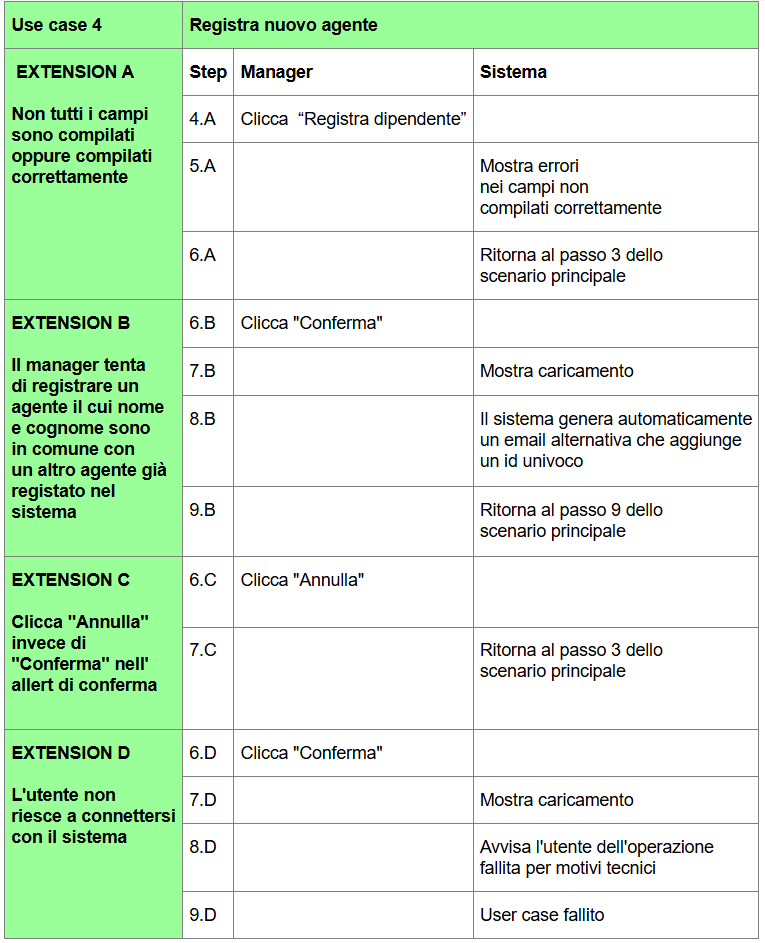
\includegraphics[width=1\linewidth]{"Immagini/cockburn/registra nuovo agente Extensions.png"}
	\caption[CockBurn extensions: registra nuovo agente]{}
	\label{fig:registra-nuovo-agente-extensions}
\end{figure}
